\documentclass[journal,12pt,twocolumn]{IEEEtran}
%
\usepackage{setspace}
\usepackage{gensymb}
\singlespacing
\usepackage[cmex10]{amsmath}
\usepackage{siunitx}
\usepackage{amsthm}

\usepackage{mathrsfs}

\usepackage{txfonts}
\usepackage{stfloats}

\usepackage{steinmetz}
\usepackage{cite}
\usepackage{cases}
\usepackage{subfig}
\usepackage{longtable}
\usepackage{multirow}
\usepackage{enumitem}
\usepackage{mathtools}
\usepackage{tikz}
\usepackage{circuitikz}
\usepackage{verbatim}
\usepackage{tfrupee}
\usepackage[breaklinks=true]{hyperref}
\usepackage{tkz-euclide} % loads  TikZ and tkz-base
\usetikzlibrary{calc,math}
\usetikzlibrary{fadings}
\usepackage{listings}
    \usepackage{color}                                            %%
    \usepackage{array}                                            %%
    \usepackage{longtable}                                        %%
    \usepackage{calc}                                             %%
    \usepackage{multirow}                                         %%
    \usepackage{hhline}                                           %%
    \usepackage{ifthen}                                           %%
  %optionally (for landscape tables embedded in another document): %%
    \usepackage{lscape}     
\usepackage{multicol}
\usepackage{chngcntr}
\DeclareMathOperator*{\Res}{Res}

\renewcommand\thesection{\arabic{section}}
\renewcommand\thesubsection{\thesection.\arabic{subsection}}
\renewcommand\thesubsubsection{\thesubsection.\arabic{subsubsection}}

\renewcommand\thesectiondis{\arabic{section}}
\renewcommand\thesubsectiondis{\thesectiondis.\arabic{subsection}}
\renewcommand\thesubsubsectiondis{\thesubsectiondis.\arabic{subsubsection}}

\hyphenation{op-tical net-works semi-conduc-tor}
\def\inputGnumericTable{}                                 %%

\lstset{
%language=C,
frame=single, 
breaklines=true,
columns=fullflexible
}
\begin{document}
%


\newtheorem{theorem}{Theorem}[section]
\newtheorem{problem}{Problem}
\newtheorem{proposition}{Proposition}[section]
\newtheorem{lemma}{Lemma}[section]
\newtheorem{corollary}[theorem]{Corollary}
\newtheorem{example}{Example}[section]
\newtheorem{definition}[problem]{Definition}
\newcommand{\BEQA}{\begin{eqnarray}}
\newcommand{\EEQA}{\end{eqnarray}}
\newcommand{\define}{\stackrel{\triangle}{=}}
\bibliographystyle{IEEEtran}
\providecommand{\mbf}{\mathbf}
\providecommand{\pr}[1]{\ensuremath{\Pr\left(#1\right)}}
\providecommand{\qfunc}[1]{\ensuremath{Q\left(#1\right)}}
\providecommand{\sbrak}[1]{\ensuremath{{}\left[#1\right]}}
\providecommand{\lsbrak}[1]{\ensuremath{{}\left[#1\right.}}
\providecommand{\rsbrak}[1]{\ensuremath{{}\left.#1\right]}}
\providecommand{\brak}[1]{\ensuremath{\left(#1\right)}}
\providecommand{\lbrak}[1]{\ensuremath{\left(#1\right.}}
\providecommand{\rbrak}[1]{\ensuremath{\left.#1\right)}}
\providecommand{\cbrak}[1]{\ensuremath{\left\{#1\right\}}}
\providecommand{\lcbrak}[1]{\ensuremath{\left\{#1\right.}}
\providecommand{\rcbrak}[1]{\ensuremath{\left.#1\right\}}}
\theoremstyle{remark}
\newtheorem{rem}{Remark}
\newcommand{\sgn}{\mathop{\mathrm{sgn}}}
\providecommand{\abs}[1]{\left\vert#1\right\vert}
\providecommand{\abs}[1]{\lvert#1\rvert} 
\providecommand{\res}[1]{\Res\displaylimits_{#1}} 
\providecommand{\norm}[1]{\left\lVert#1\right\rVert}
%\providecommand{\norm}[1]{\lVert#1\rVert}
\providecommand{\mtx}[1]{\mathbf{#1}}
\providecommand{\mean}[1]{E\left[ #1 \right]}
\providecommand{\fourier}{\overset{\mathcal{F}}{ \rightleftharpoons}}
%\providecommand{\hilbert}{\overset{\mathcal{H}}{ \rightleftharpoons}}
\providecommand{\system}{\overset{\mathcal{H}}{ \longleftrightarrow}}
	%\newcommand{\solution}[2]{\textbf{Solution:}{#1}}
\newcommand{\solution}{\noindent \textbf{Solution: }}
\newcommand{\cosec}{\,\text{cosec}\,}
\providecommand{\dec}[2]{\ensuremath{\overset{#1}{\underset{#2}{\gtrless}}}}
\newcommand{\myvec}[1]{\ensuremath{\begin{pmatrix}#1\end{pmatrix}}}
\newcommand{\mydet}[1]{\ensuremath{\begin{vmatrix}#1\end{vmatrix}}}
\numberwithin{equation}{subsection}
\makeatletter
\@addtoreset{figure}{problem}
\makeatother
\let\StandardTheFigure\thefigure
\let\vec\mathbf
\renewcommand{\thefigure}{\theproblem}
\def\putbox#1#2#3{\makebox[0in][l]{\makebox[#1][l]{}\raisebox{\baselineskip}[0in][0in]{\raisebox{#2}[0in][0in]{#3}}}}
     \def\rightbox#1{\makebox[0in][r]{#1}}
     \def\centbox#1{\makebox[0in]{#1}}
     \def\topbox#1{\raisebox{-\baselineskip}[0in][0in]{#1}}
     \def\midbox#1{\raisebox{-0.5\baselineskip}[0in][0in]{#1}}
\vspace{3cm}
\title{Assignment-2}
\author{G.Soujanya}
\maketitle
\newpage
\bigskip
\renewcommand{\thefigure}{\theenumi}
\renewcommand{\thetable}{\theenumi}
%
\section{QUESTION NO-2.14 (linear forms)}
\item Find the equation of the line satisfying the following conditions.
\begin{enumerate}
\item passing through the point \myvec{-1\\1} and \myvec{2\\-4}
\item perpendicular distance from the origin is 5 and the angle made by the perpendicular with the positive x-axis is 30$\degree$.
\end{enumerate}
%
%
\section{Solution}
\begin{enumerate}
\item Let $\vec{A}=\myvec{-1\\1}$ and $\vec{B}=\myvec{2\\-4}}$
\\
  direction vector $\vec{m}$ of the points \vec{A} and \vec{B} is give by, 

\begin{align}
\label{eq:line_norm_dir}
\vec{m}&={\vec{B}-\vec{A}}&={\myvec{3\\-5}}
\end{align}
The line parallel to the X-axis has direction vector \vec{m}=\myvec{3\\-5}.Hence its equation is obtained as
\begin{align}
\label{eq:line_norm_vec}
\vec{X}&={\myvec{-1\\1}}+\lambda{\myvec{3\\-5}}
\end{align}
\caption{plot of the line $AB$}
\numberwithin{figure}{section}
\begin{figure}[ht]
\centering
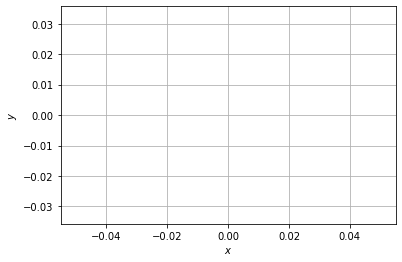
\includegraphics[width=\columnwidth]{download (1).png}
\caption{Plot of Line $AB$ (Part-1)}
\label{Plot of Line $AP$ (Part-1)}
\end{figure}
\begin{align}
    
\end{align}
%
\item   the foot of the perpendicular $P$ is the intersection of the lines $L$ and $M$.  Thus, 
\begin{align}
\label{eq:line_pt_dist_foot}
\vec{n}^T\vec{P} &= c
\\
\label{eq:line_pt_dist_foot_normal}
\vec{P} = \vec{A} + \lambda\vec{n}
\\
\text{or, } \vec{n}^T\vec{P} = \vec{n}^T\vec{A} + \lambda\norm{\vec{n}}^2 = c
\\
\label{eq:line_pt_dist_lam}
\implies -\lambda = \frac{\vec{n}^T\vec{A}-c}{\norm{\vec{n}}^2}
\end{align}


%
From \eqref{eq:line_pt_dist_lam}
%
\begin{align}
\label{eq:line_pt_dist}
\norm{\vec{P} - \vec{A}}  = \frac{\abs{\vec{n}^T\vec{A}-c}}{\norm{\vec{n}}}
\end{align}

%
\begin{align}
\vec{n} = \myvec{1\\\tan 30\degree}
\end{align}
%
$\because \vec{A} = \vec{0}$, 
\begin{align}
5 = \frac{\abs{ c}}{\norm{\vec{n}}} \implies c &= \pm 5\sqrt{1+\tan^2 30\degree} 
\\
&= \pm 5 \sec 30\degree
\end{align}
%
where 
%
\begin{align}
\sec \theta = \frac{1}{\cos \theta}
\end{align}
%
This follows from the fact that
%
\begin{align}
\cos^2 \theta + \sin^2 \theta &= 1
\\
\implies 1 + \frac{\sin^2 \theta}{\cos^2 \theta} &= \frac{1}{\cos^2 \theta}
\end{align}
%
It is easy to verify that 
%
\begin{align}
\frac{\sin \theta}{\cos \theta} &= \tan \theta
\\
\implies 1 + \tan^2 \theta &= \sec^2 \theta
\end{align}
%
$Thus$, the equation of the line is 
\begin{align}

& \myvec{1 &\tan 30\degree} \vec{c} = \pm 5 \sec 30\degree
\end{align

\numberwithin{figure}{section}
\begin{figure}[ht]
\centering
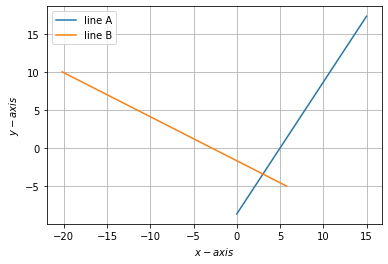
\includegraphics[width=\columnwidth]{download.png}
\caption{Plot of Line $AB$ (Part-2)}
\label{Plot of Line $LM$ (Part-2)}
\end{figure}
\end{document}
